\documentclass[__main__.tex]{subfiles}

\begin{document}

\section{Понятия табулирования линейного оператора в сепарабельном банаховом пространстве и аппроксимирования линейного уравнения, имеющего единственное решение, схемой табличных аналогов, и устойчивости этой схемы}

Рассмотрим в пространстве $Y_0$ линейное уравнение: 

\begin{equation}\label{7.1}
\hat{F} \left(x\right) = y_0
\end{equation}

где $y_0 \in \varepsilon \left(\hat{F}\right) \subseteq Y_0$ и предполагается, что уравнение \ref{7.1} имеет единственное решение $x_0 \in D\left(\hat{F}\right)$. Для пространства $Y_0$ задано аппроксимирование $\hat{p}_{\left(\cdot\right)} = \left(\hat{p}_k = \hat{\varphi}_k \circ \hat{\pi}_k\right)_{\mathbb{N}}$, где база аппроксимирования $H_{\left(\cdot\right)} = \left(H_k\right)_{\mathbb{N}}$ согласована с табулированием $\hat{\pi}_{\left(\cdot\right)} = \left(\hat{\pi}_k\right)$. Не ограничивая общности, предполагаем, что $\left|H_k\right| = k+1$, то есть $\hat{\pi}_k \in Hom \left(Y_0, {}^> \mathbb{R}^{k+1}_*\right)$, для $\forall k\in\mathbb{N}$.

Предполагаем, что $\hat{p}_{\left(\cdot\right)}$ - корректное аппроксимирование.

Рассмотрим последовательность матриц $\underline{F}_{\left(\cdot\right)} = \left(\underline{F}_{\left(k\right)} \in L \left(\mathbb{R};k+1\right)\right)_{\mathbb{N}}$, которая индуцирует последовательность табличнх операторов $\hat{\underline{F}}_{\left(\cdot\right)} = \left(\hat{\underline{F}}_{\left(k\right)} \in End\left({}^> \mathbb{R}^{k+1}_*\right)\right)$, где $\hat{\underline{F}}_{\left(k\right)} \left({}^> \underline{U}_{\left(k\right)}\right) = \underline{F}_{\left(k\right)} \cdot {}^> \underline{U}_{\left(k\right)}$ для ${}^> \underline{U}_{\left(k\right)} \in \underline{\upsilon}_{\left(k\right)}= {}^> \mathbb{R}^{k+1}_*$ и $\forall k \in \mathbb{N}$.

Для $\forall k \in \mathbb{N}$ матрицу $\underline{F}_{\left(k\right)}$ называют \textbf{табуляцией} оператора $\hat{F}$ и последовательность $\underline{F}_{\left(\cdot\right)} = \left(\underline{F}_{\left(k\right)}\right)_{\mathbb{N}}$ называют $\hat{\pi}_{\left(\cdot\right)} = \left(\hat{\pi}_k\right)_{\mathbb{N}}$ - \textbf{табулированием оператора} $\hat{F}$, если для $\forall x \in d \left(\hat{F}\right)$ выполняется условие:

$$
\| \left(\underline{\hat{F}}_{\left(k\right)} \circ \hat{\pi}_k - \hat{\pi}_k \circ \hat{F}\right) \left(x\right) \| \xrightarrow[k\rightarrow + \infty]{} 0,
$$

где $\hat{\pi}_{\left(\cdot\right)} = \left(\hat{\pi}_k \in Hom_c\left(Y_0,{}^>\mathbb{R}^{k+1}_*\right)\right)_{\mathbb{N}}$ - введённое ранее табулирование $Y_0$.

Для создания схемы табличных аналогов уравнения \ref{7.1} испольуем схему диаграмм отображений.

\begin{figure}[h!]
	\centering
	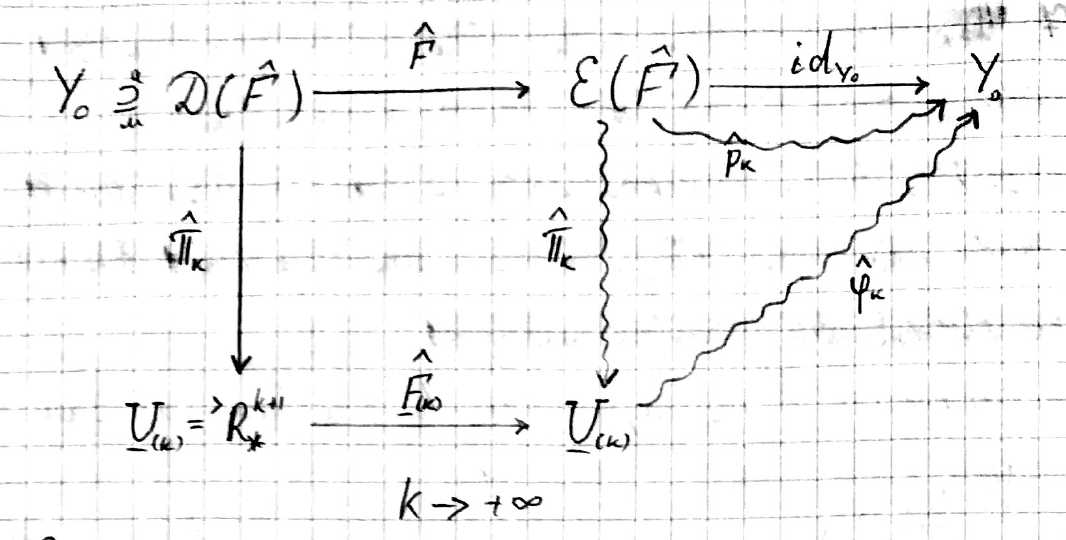
\includegraphics[width=0.7\linewidth]{img/img_7_1}
	\caption{}
	\label{fig:img71}
\end{figure}

Согласно схеме диаграмм отображений на рисунке, схему табличных аналогов уравнения \ref{7.1} представляем в виде:

\begin{equation}\label{7.2}
\begin{cases}
\underline{\hat{F}}_{\left(k\right)} \cdot {}^> \underline{U}_{\left(k\right)} = {}^> \underline{\upsilon}_{\left(k\right)} = \hat{\pi}_k \left(y_0\right)\\
k\rightarrow+\infty
\end{cases}
\end{equation}

Говорят, что схема \ref{7.2} \textbf{аппроксимирует уравнение} \ref{7.1}, если последовательность $\underline{F}_{\left(\cdot\right)} = \left(\underline{F}_{\left(k\right)}\right)_{\mathbb{N}} \pi_{\left(\cdot\right)}$ - табулирует оператор $\hat{F}$.

Ранее предполагалось, что $x_0 \in D\left(\hat{F}\right)$ - единственное решение уравнения \ref{7.1}. Если последовательность $\underline{F}_{\left(\cdot\right)}\pi_{\left(\cdot\right)}$  - табулирует оператор $\hat{F}$, то для схемы \ref{7.2} получаем 

\begin{equation}
\begin{cases}
\underline{F}_k \cdot \hat{\pi}_k \left(x_0\right) = \hat{\pi}_k \left(y_0\right)+ {}^>\underline{\varepsilon}_{\left(k\right)} \\
\lim_{k\rightarrow + \infty} \| {}^>\underline{\varepsilon}_{\left(k\right)} \| = 0
\end{cases}
\end{equation}

поскольку $\hat{\pi}_k \left(y_0\right) = \pi_k \left(\hat{F}\left(x_0\right)\right) = \hat{\pi} \circ \hat{F} \left(x_0\right)$ для $k\in\mathbb{N}$.

Говорят, что схема \ref{7.2} \textbf{устойчива}, если для $\forall k \in\mathbb{N}$ выполняется условие: $\exists \underline{F}^{-1}_{\left(k\right)}$ и последовательность $\left(\| \underline{F}^{-1}_{\left(k\right)} \|\right)_{\mathbb{N}} = \left(\underline{\hat{F}}^{-1}_{\left(k\right)}\right)_{\mathbb{N}}$- ограничена.

\end{document}
